% Chapter Template

\chapter{Ergebnisse} % Main chapter title

\label{Kaptiel4} % Change X to a consecutive number; for referencing this chapter elsewhere, use \ref{ChapterX}

%----------------------------------------------------------------------------------------
%	SECTION 1
%----------------------------------------------------------------------------------------
\section{Versuchsaufbau}
Für die Ausführung der Anfragen wurde die Dell Precision Workstation T5500 verwendet. Das System besitzt 16 Prozessorkerne vom Typ Intel Xeon  X5500 mit je 2,66 GHz und  8 MB Level3 Cache. Insgesamt stehen 72 GB DDR3 RAM mit 1333 MHz zur Verfügung und das System läuft auf Ubuntu 18.04. Alle Datensätze werden auf einer SEAGATE ST3250318AS Festplatte mit insgesamt 250 GB Kapazität, 8 MB Cache und 7200 Umdrehungen pro Minute gespeichert.\newline
 Jede Anfrage des ersten Testlaufes wurde 50 mal ausgeführt und die Anfragen des zweiten Testlaufes wurden 25 mal ausgeführt. In OrientDB wurden alle Anfragen 25 mal wiederholt. Als repräsentativer Wert für die Bearbeitungszeit einer Anfrage  wurde das Arithmetische Mittel aus allen Wiederholungen gewählt. Bei der Berechnung wurde die Zeit für die allererste Ausführung einer Anfrage nicht berücksichtigt, da durch das Caching eine unverhältnismäßig hohe Bearbeitungszeit beim ersten Ausführen beobachtet wurde. In OrientDB ist die erste Bearbeitungen der Anfrage im Durschnitt ca. 43\% langsamer, als die Wiederholungen  der Anfragen. In Neo4j ist die erste Bearbeitung mit Cypher ca. 40 \% langsamer und mit der Core API ca. 17\% langsamer.  
\section{Auswertung}
Im folgenden Abschnitt werden Bearbeitungszeiten der Testläufe in Millisekunden tabellarisch präsentiert.  Darauf aufbauend werden die Hypothesen aus Kapitel 3 überprüft.  
\subsection{Ergebnisse des ersten Testlaufes}
Die Ergebnisse für Grundanfrage 1.1.1
\begin{Verbatim}[frame=single]
MATCH (X:Person)-[:RELATIONSHIP3]->(Y:Person) 
WHERE X.attribute>=250 AND Y.attribute>=15  
RETURN COUNT(DISTINCT(Y))
\end{Verbatim} 
 werden  in Tabelle \ref{tab:Query1_1} gezeigt. Durch die Bedingungen im Where-Prädikat entstehen im Vergleich zu den darauffolgenden Anfragen relativ hohe Bearbeitungszeiten. Die benötigte Bearbeitungszeit ist in allen drei Szenarien am längsten, wenn die Relationen in beide Richtungen betrachtet werden. Dies ist auf die hohe Anzahl der vorhandenen Relationen zurückzuführen. Bei der Anfrage in Cypher und der Core API für die RELATIONSHIP3  ist die Bearbeitungszeit bei der Suche für beide Richtungen länger als die Suchen für ausgehende und eingehende Kanten addiert. Für die Anfragen mit RELATIONSHIP3 ist die Zeit am geringsten, wenn die ausgehenden Kanten betrachtet werden. \newline
Die Anfrage für RELATIONSHIP3 wird mit der Core API in  allen Fällen fast doppelt so schnell berechnet wie in Cypher. Dieses Verhalten wird bei den weiteren Grundanfragen ebenfalls erwartet, da die Core API sehr nah an den Kernfunktionen von Neo4j arbeitet. \newline
Die Anfragen werden in Cypher für RELATIONSHIP2 etwas mehr als 1000 mal schneller als für REALTIONSHIP3 bearbeitet. Dies deutet auf eine gute Skalierbarkeit des Systems hin, da die Berechnungen beinahe linear zu der Anzahl der zu betrachtenden Relationen ansteigen. 
\FloatBarrier  
\begin{table}[h]
\centering
\begin{tabular}{ |p{3cm}||p{3cm}|p{3cm}|p{3cm}|  }
	\hline
	Anfrage& RELATIONSHIP3 &Core API&RELATIONSHIP2\\
	\hline
	Ausgehend	& 212620  & 82057   & 160\\
	Eingehend   & 215383    &123963&  64\\
	Beides&496704 & 222150&  165\\
	\hline
\end{tabular}
\caption{Ergebnisse der Grundanfrage 1.1.1}
\label{tab:Query1_1}
\end{table}
\FloatBarrier
 \noindent Die beobachteten Zeiten für Grundanfrage 1.2
 \begin{Verbatim}[frame=single]
 MATCH (p:Person {name:'Person613'}) return p
 \end{Verbatim} 
  in Tabelle \ref{tab:Query1_2} sind im Vergleich zu den Zeiten der anderen Grundanfragen sehr gering. Durch die geringe Anzahl von 50004 Knoten,dem Verwenden von Indizes und der konstanten Zugriffszeit entstehen die geringen Zeiten. \newline Entgegen der Hypothese entsteht ein hoher zeitlicher Unterschied, wenn sich die Bedingung im Where-Prädikat statt im Match-Prädikat 	befindet. Die beobachtete Bearbeitungszeit bei der Anfrage mit der Bedingung in dem Where-Prädikat ist drei mal schneller, als bei der Anfrage mit der Bedingung im Match-Prädikat. Da der Cypher Query Optimizer alle Bedingungen des Match-Prädikates in ein Where-Prädikat verschiebt, wird hier gezeigt, dass dieser Optimierungsschritt selber eine  Berechnungszeit in Anspruch nimmt. Für ein optimalen Gebrauch von Neo4j sollten dementsprechend alle Bedingungen direkt in einem Where-Prädikat formuliert werden, dies wird auch von den Entwicklern empfohlen \parencite{Optimizer}. \newline
In diesem Fall wird die Traversal API nicht genutzt, sondern nur die Core API. Eine Kernfunktion namens $findNodes()$ übernimmt die Suche nach einem Knoten mit angegebenen Eigenschaften, ohne dass der Nutzer das Vorgehen spezifizieren muss.  
\FloatBarrier
\begin{table}[h]
	\centering
		\begin{tabular}{ |p{3cm}|p{3cm}|p{3cm}|p{3cm}|  }
			\hline
			Ohne Where& Mit Where& Core API  \\
			\hline
			1,69   &  0,54  & 0,29  \\
			\hline
		\end{tabular}
		\FloatBarrier
		\caption{Ergebnisse der Grundanfrage 1.2}
		\label{tab:Query1_2}
\end{table}
 \vskip 2.5cm
\noindent Für Grundanfrage 1.3
\begin{Verbatim}[frame=single]
MATCH (X:Person{name: 'Person1'})-[:Relationship3]->(n1) 
WITH COLLECT(n1) as n 
MATCH (Y:Person{name: 'Person2'})-[:Relationship3]->(n1) 
WHERE n1 in n
RETURN COUNT(DISTINCT(n1))
\end{Verbatim} 
 wurde beobachtet, dass die semantisch äquivalente Anfrage ca. 1,57 mal schneller bearbeitet wird. Dies ist auf die effiziente Implementierung des IN-Operators zurückzuführen. Wie bei Grundanfrage 1.1.1 ist die Bearbeitung in der Core API schneller als in Cypher.
Die genauen Ergebnisse befinden sich in Tabelle	\ref{tab:Query1_3}.
\FloatBarrier
\begin{table}[h]
	\centering
		\begin{tabular}{ |p{3cm}|p{3cm}|p{3cm}|p{3cm}|  }
			\hline
			Grundanfrage & Äquivalent&Core API\\
			\hline
			 13,36    & 8,66 &  3,2\\
			\hline
		\end{tabular}
		\caption{Ergebnisse der Grundanfrage 1.3}
		\label{tab:Query1_3}
\end{table}
\FloatBarrier

\noindent Die normierte Verteilung aller Bearbeitungszeiten der Grundanfragen des ersten Testlaufes und ihrer Umformulierungen werden in Abbildung \ref{ref:Compare1} dargestellt. 

\begin{center}
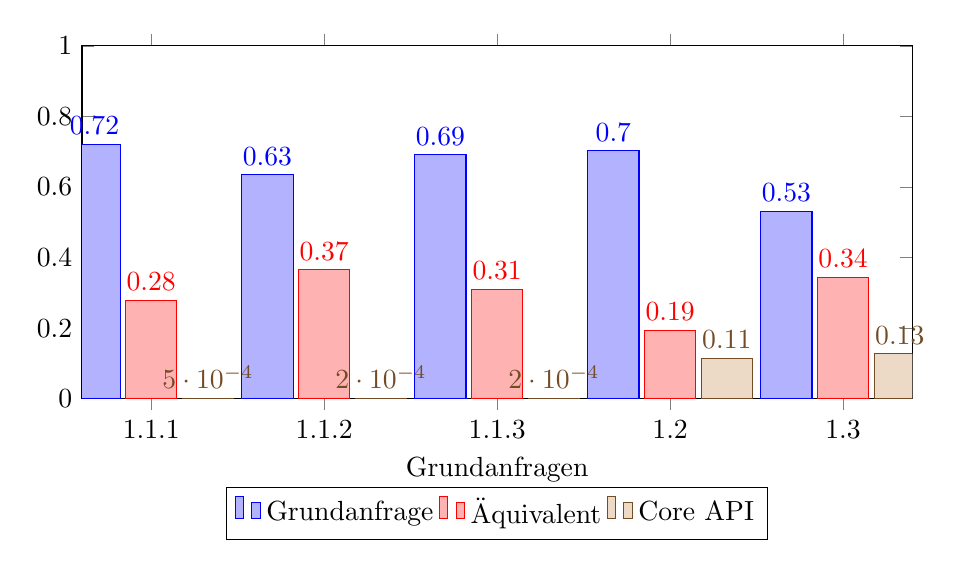
\begin{tikzpicture}
\centering
  \begin{axis}[
ybar,
bar width=.65cm,
width=\textwidth,
height=.5\textwidth,
legend style={at={(0.5,-0.25)},
	anchor=north,legend columns=-1},
symbolic x coords={1.1.1,1.1.2,1.1.3,1.2,1.3},
xtick=data,
nodes near coords,
nodes near coords align={vertical},
ymin=0,ymax=1,
xlabel={Grundanfragen},
]

\addplot coordinates {(1.1.2,0.6345) (1.1.1,0.7211)(1.1.3,0.6908)(1.2,0.7025) (1.3,0.5297)};
\addplot coordinates {(1.1.2,0.3652) (1.1.1,0.2783)(1.1.3,0.3089)(1.2,0.1935) (1.3,0.3434)};
\addplot coordinates{(1.1.2,0.0002)(1.1.1,0.0005)(1.1.3,0.0002)(1.2,0.1139)(1.3,0.1269)};
\legend{Grundanfrage,Äquivalent,Core API}
\end{axis}
\end{tikzpicture}
\captionof{figure}{Übersicht der Anfragen aus dem ersten Testlauf} 
\label{ref:Compare1}
\end{center}
\FloatBarrier

\subsection{Ergebnisse des zweiten Testlaufes}
In der Grundanfrage 2.1.1
\begin{Verbatim}[frame=single]
MATCH(p:Person{name:'Person1'})-[:RELATIONSHIP3*2]->(p1:Person) 
RETURN COUNT(DISTINCT(p1))
\end{Verbatim}
 werden bei der Traversierung in der Tiefe zwei ausgehend von Person1 99 \% aller Knoten des Graphen erreicht. Bei der Tiefe drei werden 100 \% der Knoten erreicht. Wie Tabelle \ref{tab:Query2_1} zeigt, wird mit Cypher die Traversierung in die Tiefe zwei ca. 64 mal schneller ausgeführt als die Traversierung in die Tiefe drei. In der Core API benötigt die Traversierung in die Tiefe drei mit der Breitensuche ca. 18 mal mehr Zeit als in die Tiefe zwei. Mit Verwendung der Tiefensuche benötigt die tiefere Traversierung nur 1,2 mal mehr Zeit. Da die Anzahl der zu betrachtenden Knoten um der Faktor 2500 ansteigt, besteht in allen Fällen kein linearer Zusammenhang zwischen der Bearbeitungszeit und der Anzahl der Knoten, die betrachtet werden müssen. \newline 
Es wird bestätigt, dass die Anfrage mit Tiefensuche  schneller als die Anfrage mit Breitensuche ausgeführt wird, in diesem Fall wird die Tiefensuche für Anfrage in der Tiefe zwei ca.18,4 mal schneller als Anfrage mit der Breitensuche ausgeführt. In der Tiefe drei wird die Tiefensuche ca. 277 mal schneller als die Breitensuche ausgeführt. Dies wird in Kapitel drei durch das Verhältnis der Breite zur Tiefe begründet. 
\FloatBarrier
\begin{table}[h]
\centering
		\begin{tabular}{ |p{3cm}||p{3cm}|p{3cm}|p{3cm}|  }
			\hline
			Anfrage& Cypher & Breitensuche&Tiefensuche\\
			\hline
			Tiefe 2   & 3501    & 1545&   84\\
			Tiefe 3&    223556  & 28318   & 102\\
			\hline
		\end{tabular}
		\caption{Ergebnisse der Grundanfragen 2.1.1 und 2.1.2}
		\label{tab:Query2_1}
\end{table}
\FloatBarrier
\noindent Wie Tabelle \ref{tab:Query2_2} zeigt, besteht ein geringer Unterschied zwischen Grundanfrage 2.2
\begin{Verbatim}[frame=single]
MATCH t=(p:Person{name :'Person1'})-[:RELATIONSHIP3]->(p1:Person)
-[:RELATIONSHIP3]->(p2)
WHERE NOT (p)-[:RELATIONSHIP3]->(p2) 
RETURN COUNT(DISTINCT(p2))
\end{Verbatim} 
 und der äquivalenten Anfrage in Cypher. Beide Anfragen sind um ein vielfaches langsamer als die Anfrage, die die Core API verwendet. In der Core API Anfrage werden zwei Ergebnismengen vom Java-typ Set gebildet und durch den Aufruf der Funktion removeAll() werden die Elemente der einen Mengen aus der anderen Menge entfernt. Dies entspricht einer Realisierung des Where not Ausdrucks in Java und wird schneller ausgeführt als der Ausdruck in Cypher. Alle drei Anfragen besitzen im Vergleich zu vorangegangen Anfragen eine extrem hohe Bearbeitungszeit.
\FloatBarrier
\begin{table}[h]
	\centering
		\begin{tabular}{ |p{3cm}|p{3cm}|p{3cm}|p{3cm}|  }
			\hline
			Grundanfrage 2.2 & Äquivalent&Core API\\
			\hline
			4740646    & 4753414 &  1609\\
			\hline
		\end{tabular}
		\caption{Ergebnisse der Grundanfrage 2.2}
		\label{tab:Query2_2}
\end{table}
\FloatBarrier
\noindent Der kürzeste Pfade, welcher in Grundanfrage 2.3
\begin{Verbatim}[frame=single]
MATCH (p:Person{name :'Person1'}),(p1:Person{name :'Person42'}),
path=shortestPath((p)-[:RELATIONSHIP4*..3]->(p1)) 
RETURN LENGTH(path)
\end{Verbatim} 
 untersucht wird, besitzt die Länge zwei. Die Grundanfrage 2.1.1 zeigt, dass bei einer Pfadlänge von zwei die meisten Knoten ausgehend von Person1 erreicht werden. Wie Tabelle \ref{tab:Query2_3} zeigt, ist die benötigte Bearbeitungszeit der Anfrage in Cypher unter Verwendung des gegebenen Algorithmus geringer als alle anderen Grundanfragen außer Grundanfrage 1.2. Erstmalig wird die Anfrage in Cypher schneller als die Formulierung in der Core API bearbeitet. Die Anfrage wird in Cypher 1,37 mal schneller beantwortet und  der absolute Unterschied zwischen den Bearbeitungszeiten beträgt 3,1 ms. Durch die geringe absolute Differenz ist es nicht garantiert, dass der kürzeste Pfad immer am schnellste mit Cypher berechnet wird. \newline
Die äquivalente Formulierung in Cypher besitzt die höchste aller beobachtetet Bearbeitungszeiten der gestellten Anfragen in Neo4j mit ca. 2,3 Stunden. Diese Formulierung ist eine naiver Ansatz ohne Verwendung des Algorithmus und besitzt viele Berechnungsschritten, die durch den Algorithmus entfallen. Zudem stoppt der Limit-Ausdruck nicht vorzeitig die Berechnung, sondern filtert die Ergebnismenge erst nach der Berechnung, dieses Verhalten ist mit der konservativen Stop-Strategie aus SQL zu vergleichen\parencite{carey1997saying}.   
\FloatBarrier
\begin{table}[!htb]
	\centering
		\begin{tabular}{ |p{3cm}|p{3cm}|p{3cm}|p{3cm}|  }
			\hline
			Grundanfrage 2.3 & Äquivalent&Core API\\
			\hline
			8,4    & 8370298 &  11,5\\
			\hline
		\end{tabular}
		\caption{Ergebnisse der Grundanfrage 2.3}
		\label{tab:Query2_3}
\end{table}
\FloatBarrier
\noindent Die Ergebnisse der Traversierungen des gesamten Graphen, wie in Grundanfrage 2.4.1
 \begin{Verbatim}[frame=single]
MATCH (a)-[RELATIONSHIP4]->(b) RETURN COUNT(DISTINCT(b))
\end{Verbatim}
 werden in Tabelle \ref{tab:Query2_4} dargestellt.
 In der Core API ist die bidirektionale Traversierung mit Breitensuche ca. 1,15 mal schneller als der gleiche Algorithmus bei einer einseitige Traversierung. Bei der Tiefensuche ist die bidirektionale Suche ca. 1,04 mal schneller. In beiden Fällen sind die einseitigen Traversierungen langsamer als die bidirektionale Alternativen. \newline
Trotz einer semantischen Äquivalenz von Grundanfrage 2.4.1 mit der Grundanfrage 2.1.2, bei der alle Knoten erreicht werden, ist eine höhere Bearbeitungszeit zu beobachten. 
\FloatBarrier
\begin{table}[!htb]
	\centering
	\begin{tabular}{ |p{5cm}||p{3cm}|p{3cm}|p{3cm}|  }
		\hline
		Anfrage & Zeit\\
		\hline
		Grundanfrage 2.4.1 & 284594\\
		\hline
		Vergleichsanfrage 1 & 31020  \\
		\hline
		Grundanfrage 2.4.2 & 31050\\
		\hline
		Grundanfrage 2.4.3 &   26982 \\
		\hline
		Grundanfrage 2.4.4 &  29558\\
		\hline
	\end{tabular}
	\caption{Ergebnisse der Grundanfragen 2.4.1-2.4.4}
	\label{tab:Query2_4}
\end{table}
\FloatBarrier

\subsection{Ergebnisse des dritten Testlaufes}
Für die folgenden Aussagen werden die Werte aus der Tabelle \ref{tab:Query3}  betrachtet. Diese Tabelle stellt die Bearbeitungszeiten der Grundanfragen, ihrer Äquivalente in der Core API und in der OrientDB dar. \newline
Die Grundanfragen 1.1.1-1.1.3 werden in Cypher durchschnittlich ca. 12 mal schneller ausgeführt als in der OrientDB, die relativ langen Bearbeitungszeiten bei beiden Systemen entstehen durch die Bedingungen im Where-Prädikat. In allen Fällen benötigt die Grundanfrage 1.1.3, welche die eingehenden und ausgehenden Kanten betrachtet, die längste Zeit zur Bearbeitung. Dies zeigt, dass OrientDB und Neo4j durch das Einfügen einer Bedingung im Where-Prädikat und der Anzahl der zu betrachtenden Kanten beeinflusst werden und bei solchen Anfragen aufwendige Berechnungen ausführen. \newline
 Grundanfrage 1.2, welche solange über den Graphen traversiert bis ein gegebener Knoten gefunden ist, weist in OrientDB eine schnellere Bearbeitungszeit als Neo4j mit der Core API oder Cypher auf und wird ca. 3,7 mal schneller bearbeitet als die in Cypher gestellte Anfrage. Dies lässt sich mit einer effizienteren Implementierung der Indizies erklären. Die Anfrage wird in allen Fällen in weniger als einer Millisekunde beantwortet und bildet die am schnellsten beantwortete Anfrage. \newline
Grundanfrage 1.3, welche eine einfache Anfrage zum Finden von gemeinsamen Nachbarn darstellt, besitzt in Cypher und der Core API eine relativ geringe Bearbeitungszeit in der Größenordnung von einigen Millisekunden. In OrientDB befindet sich Grundanfrage 1.3 mit einer benötigten Zeit von 83955 ms in einer anderen Größenordnung und deutet darauf hin, dass der Vergleich von zwei Mengen miteinander in Neo4j effizienter implementiert ist. Dies ist auch in Grundanfrage 2.2 zu beobachten, für diese Anfrage muss bis in die Tiefe zwei traversiert werden und zwei Mengen müssen miteinander verglichen werden. Die Anfrage besitzt eine extrem hohe Bearbeitungszeit von mehreren Stunden, obwohl das Traversieren in der Tiefe zwei, wie bei Grundanfrage 2.1.1 mit 72092 ms zu beobachten, eine relativ geringe Zeit benötigt, der Vergleich der beiden Mengen bildet so den rechenaufwendigeren Schritt. \newline
 Grundanfrage 2.1.1 wird in Cypher ca. 20,6 mal schneller bearbeitet als in der OrientDB. Grundanfrage 2.1.2 wird in der OrientDB ca. 2,1 mal schneller beantwortet. Dies deutet darauf hin, dass OrientDB besser skaliert als Neo4j mit Cypher. In OrientDB wird die Grundanfrage 1.1.2 ca. 1,5 mal langsamer ausgeführt als Grundanfrage 1.1.1, in Neoj4 wird diese Anfrage ca. 60,9 mal langsamer ausgeführt.   Die Grundanfrage 2.1.2 ist mit der Grundanfrage 1.2 die einzige Grundanfrage, die in OrientDB schneller bearbeitet wird, als in Neo4j mit Cypher. \newline  
 Grundanfrage 2.2 konnte in dieser Evaluation nicht vollständig analysiert werden, da die erste Ausführung der Anfrage ohne Caching ungefähr 70 Stunden benötigt hat. Weitere Wiederholungen mit Caching waren nicht möglich, aber würden bei der durchschnittlichen Verkürzung der Bearbeitungszeit durch das Caching von ca. 43\%  ungefähr 40 Stunden benötigen . \newline
OrientDB benötigt mit 37,6 ms für Grundanfrage 2.3  wie Neo4j eine relativ kurze Zeit von einigen Millisekunden zur Bearbeitung, dies lässt sich durch eine effiziente Implementierung des shortestpath-Algorithmus erklären. Das Finden des kürzesten Pfades ist ein grundlegendes Problem bei Graphen und der Algorithmus wurde bereits in der OrientDB Version 1.7.8 vom 13. August 2014 veröffentlicht \parencite{Old_OrientDB}. Durch die frühe Zurverfügungstellung ist es wahrscheinlich, dass der Algorithmus mit einer effizienten Implementierung veröffentlicht wurde oder über die Jahre optimiert wurde. \newline
Für die Grundanfrage 2.4.2, welche mit Breitensuche über den gesamte Graphen traversiert, ist nur ein Vergleich zwischen OrientDB und der Core API von Neo4j möglich, da der Such-Algorithmus in Cypher nicht explizit angegeben werden kann und immer Tiefensuche verwendet wird. Durch die gleiche Komplexität von O(V+E) bei der Tiefen- und Breitensuche, benötigen die Grundanfragen 2.4.1 und 2.4.2 in OrientDB eine gleich lange Bearbeitungszeit. In Cypher wird die Grundanfrage 2.4.1 ca. 2,7 mal schneller bearbeitet als die gleiche Anfrage in OrientDB. Mit Verwendung der Core API wird die einseitige Tiefen- und Breitensuche durchschnittlich ca. 24.8 mal schneller beantwortet als in OrientDB. \newline
 Unter der Berücksichtigung aller beobachteten Zeiten außer von Grundanfrage 2.2 werden die Anfragen mit der Core API durchschnittlich ca. 207 mal schneller bearbeitet als in OrientDB und mit Cypher ca. 1,9 mal schneller als OrientDB. 
\FloatBarrier
\begin{table}[h]
	\centering
	\begin{tabular}{ |p{6cm}||p{2cm}|p{2cm}|p{2cm}|  }
		\hline
		Anfrage& Cypher & OrientDB & Core API \\
		\hline
	Grundanfrage 1.1.1  & 215383 & 3495459    &  64\\
	Grundanfrage 1.1.2& 212620 & 1674758   & 160   \\
	Grundanfrage 1.1.3& 496704 & 6350806 & 165  \\
	Grundanfrage 1.2& 0,54 & 0,17   & 0,29   \\
	Grundanfrage 1.3 & 8,66& 83955  & 3,2    \\
	Grundanfrage 2.1.1& 3501 & 72092   & 84   \\
	Grundanfrage 2.1.2& 234132& 110064  & 102    \\
	Grundanfrage 2.2& 4740646 &  $\approx$ 40h   & 1609  \\
	Grundanfrage 2.3& 8,4  & 37,6   & 11,5   \\
	Grundanfrage 2.4.1& 284594 & 768830  & 31050\\
	Grundanfrage 2.4.2& -  & 774040   & 31020   \\
		\hline
	\end{tabular}
	\caption{Ergebnisse der Grundanfragen auf Neo4j und OrientDB}
	\label{tab:Query3}
\end{table}
\FloatBarrier
\section{Anwendungsszenario}
Neoj4 Inc. stellt zahlreiche Nutzungen von Graphen in verschiedenen Themenkomplexen vor \parencite{Examples}. Für jeden Themenkomplex werden mehrere Beispielgraphen von eigenständigen Entwicklern, welche nicht für Neo4j arbeiten, zur Verfügung gestellt. Das folgende Anwendungsszenario stellt den Zweck einer Graphdatenbank für Kinofilme dar.\newline
In diesem Beispiel ist der Nutzer ein Betreiber eines Kinos, welches aktuelle Kinofilme ausstrahlt und spezielle Veranstaltungen bietet. Bei diesen Veranstaltungen werden mehrere Filme von einer Kategorie oder einem bestimmten Schauspieler oder Regisseur gezeigt. Diese Veranstaltungen werden mehrere Wochen vor dem Veranstaltungstermin verplant und finden über mehrere Tage statt. Solche Veranstaltungen wurden schon mehrmals betrieben und die Planung besitzt einen routinierten Ablauf, sodass viele Schritte effizient bearbeitet werden. Der zeitaufwendigste Arbeitsschritt, stellt das Finden von Filmen für das Veranstaltungsprogramm dar. \newline
Aktuell stellt der Kinobetreiber eine Liste von Filmen für die Veranstaltung manuell zusammen, hierfür werden Filme ausgewählt, die der Betreiber selber kennt und es werden verschiedene Quellen aus dem Internet für eine Auswahl verwendet. Die Liste besitzt die Namen der Filme, zusätzliche Informationen wie die Länge eines Filmes sind durch die Vielzahl von Quellen nicht immer vorhanden. Fehlende Informationen müssen für eine optimale Planung des Kinoprogramms erneut herausgesucht werden und einige Filme müssen nach dem initialen Aufstellen der Liste  aussortiert werden. \newline  
Für eine Beschleunigung dieses Arbeitsschrittes kann Neo4j verwendet werden. Unabhängig von dem Betriebssystem steht die kostenfreie Anwendung $Neo4j\; Desktop$ zur Verfügung. Durch diese Anwendung für den Desktop ist die Bedienung von Neo4j über ein grafischen User Interface(GUI) möglich. Zusätzlich wird die Erweiterung $APOC$ benötigt, welche per Mausklick in $Neo4j\; Dekstop$ eingebunden werden kann. Mit dieser Erweiterung ist es möglich Daten mit verschiedenen Dateiformaten wie CSV oder JSON in die lokale Neo4j Datenbank zu importieren. Für das Thema Kino stehen im Internet zahlreiche, große Datensätze mit Filmen kostenfrei zur Verfügung \parencite{Kaggle}. Nach dem Importieren eines solchen Datensatzes, kann der Nutzer durch die Eingabemaske eine Anfrage stellen, um so eine übersichtliche vollständige Liste von Filme zu erhalten. Folgende Anfrage erstellt eine Liste von 20 Filmen mit dem Thema Verbrechen: 
\begin{Verbatim}[frame=single]
MATCH(m:Film) 
WHERE m.Genre = 'Verbrechen' or m.Plot contains 'Verbrechen'
RETURN m.Name as Name, m.Regie as Regie, 
	m.Länge as Länge, m.Plot as Plot 
LIMIT 20
\end{Verbatim}
Bei einem hohen Erfolg der Veranstaltung können ausgehend von den gezeigten Filmen Schauspieler aus diesen Filmen gefunden werden:
\begin{Verbatim}[frame=single]
MATCH (s:Schauspieler)-[SpielteIn]->(m:Film)
WHERE m.Genre = 'Verbrechen' or m.Plot contains 'Verbrechen'
RETURN s.Name as Name, count(m) as Anzahl_der_Filme,
Order by count(m) desc
LIMIT 10
\end{Verbatim}
Es werden 10 Schauspieler gefunden, die in den meisten Filmen zum Thema Verbrechen mitgespielt haben. Diese Schauspieler sind potenzielle Kandidaten für eine Veranstaltung, bei der nur Filme von diesen Schauspielern gezeigt werden. Durch Bedingungen bezüglich eines Attributes wie der Bewertung eines Filmen, kann die Auswahl weiter eingegrenzt werden.
\begin{Verbatim}[frame=single]
MATCH (s:Schauspieler)-[SpielteIn]->(f:Film) 
WHERE s.name = 'Christian Bale' AND f.Bewertung >= 5
RETURN f.Name as Name, f.Regie as Regie, 
	f.Länge as Länge, f.Plot as Plot 
LIMIT 20
\end{Verbatim}
Neo4j übernimmt die Auswertung eines Datensatzes, der in einem CSV Format dargestellt wird und von dem Nutzer nicht schnell verwendet werden kann. Durch die effiziente Implementierung von Neo4j wird in kurzer Zeit eine vollständige Liste mit Filmen erstellt. Der Arbeitsschritt zum Erstellen einer Liste mit geeigneten Filmen wird damit beschleunigt und effizienter ausgeführt.
\section{Limitierungen und zukünftige Arbeit}
Die durchgeführte Evaluation nutzt mit OrientDB  eine einzige Referenzdatenbank. Dies ist keine reine GDB und unterstützt eine erweiterte Verwaltung der Daten. Für eine näherer Einordnung der Performanz von Neoj4 ist ein Vergleich mit einer reinen GDB wie beispielsweise der Sparksee Database sinnvoll \parencite{Sparksee}. Diese Datenbank konnte in dieser Evaluation auf Grund von Kommunikationsprobleme mit Sparsity technologies nicht verwendet werden. Durch einen Vergleich mit der Sparksee Database könnte die Performanz von zahlreichen Graphalgorithmen  wie Zentralitäts-Algorithmen, zur Erkennung von Gruppen mit gemeinsamen Eigenschaften, überprüft werden. Dies ist mit OrientDB nicht möglich, da keine vergleichbare Implementierung der von Neo4j unterstützen Graphalgorithmen im vollen Ausmaß in OrientDB gegeben ist. \newline 
Ein Vergleich zwischen Neo4j und einer relationalen Datenbank, wie in \parencite{vicknair2010comparison} beschrieben, ist für eine weitere Beschreibung der Vor- und Nachteile einer GDB sinnvoll. Dieser Vergleich wurde aus zeitlichen Gründen nicht vollzogen. Die Referenz zur OrientDB hat einen Vergleich zu einer anderen noSQL-Datenbank dargestellt und so ein erste Einschätzung zu der Performanz von Neo4j ermöglicht. \newline
Ein weitere zu betrachtender Aspekt, ist das Ausführen einer Neo4j Datenbank im Server Modus auf mehreren Geräten verteilt. Durch diesen Aspekt können die ACID und CAP Eigenschaften untersucht werden und die Grenzen einer verteilten Neo4j-Datenbank getestet werden. Zudem kann ein Vergleich zwischen der Datenbank im eingebetteten Modus und dem Server Modus durchgeführt werden. So können Vor- und Nachteile und  Anwendungsszenarien spezifiziert werden. \newline
Eine kleinerer nicht betrachteter Aspekt ist die temporale Eigenschaft von Neo4j. Der vorgestellte Datensatz besitzt ein Attribut vom Typen Date und stellt so eine temporale Datenbank dar, es fehlt ein Testlauf mit Anfragen zu diesem Attribute. Eine Allgemeine Betrachtung des temporalen Verhalten der Datenbank ist für eine genauere Einordnung von Neo4j im Vergleich zu anderen temporalen Graphdatenbanken sinnvoll.   \newline
Die Anfragesprache GraphQL wird als standardisierte Anfragesprache für GDBs angesehen \parencite{GraphQL}. In der Zukunft sollte GraphQL auch in Neo4j getestet werden, dies ist mit einer Erweiterung für Neo4j möglich und erfordert die Verwendung einer weiteren API. In dieser Evaluation wurde GraphQL nicht verwendet. 
\section{Fazit}
Neo4j unterstützt mit den Java-Standardtypen und zahlreichen zeitlichen Typen wie Time, LocalTime oder DateTime eine Vielzahl von Datentypen, welche für die Modellierungen von Daten notwendig sind \parencite{Types}. Durch die Zurverfügungstellung der Anwendungen Neo4j Dekstop und Neo4j Browser und einer dazu gegebenen Anfragesprache, werden die benötigten Kenntnisse zur Bedienung des System minimiert. Für eine spezifischeren Gebrauch der Datenbank, werden mehrere Programmiersprachen unterstützt. Durch diese Schnittstellen ist es mögliche, das System auf viele Weisen zu nutzen und eine große Zielgruppe kann das System für viele Zwecke verwenden. \newline 
Der erste und zeite Testlauf zeigen, dass dem Gebrauch der APIs in fast allen Fällen zu einer besseren Performanz führt. Mit Verwendung der Traversal API besitzt der Nutzer eine flexible Möglichkeit die Performanz seiner Anfragen zu beeinflussen. So ist es möglich zwischen Breiten- und Tiefensuche zu wählen. Die am schnellsten bearbeiteten Anfragen besitzen keine gemeinsame Kategorie von den vorgestellten Kategorien aus Absatz \ref{Kategorien}. Die am langsamsten bearbeiteten Anfragen besitzen ebenfalls keine gemeinsamen Kategorien. Grundanfrage 2.2, welche die einzige Mustervergleichs-Anfrage ist, besitzt eine besonders hohe Bearbeitungszeit. Dementsprechend lässt sich nur für Mustervergleichs-Anfragen ein Bezug von Anfragen-Kategorie und Bearbeitungszeit in Neo4j erkennen, die anderen Kategorien weisen keinen solchen Bezug auf. \newline
Wie die Tabellen \ref{tab:Query1_2} und \ref{tab:Query2_3} zeigen, können semantisch gleiche Anfragen in Cypher Unterschiede in ihrer Performanz aufzeigen. Dieses Verhalten ist in den APIs ebenfalls zu beobachten. Das System lässt sich durch eine hohe Anzahl von Schnittstellen leicht benutzen, aber das System effektiv zu nutzen und eine Anfrage effizient ausführen zu lassen, ist nicht trivial und erfordert technologische Kenntnisse. Durch Hinweise von Neo4j Inc. werden einige Möglichkeiten für das effiziente Ausführen gegeben \parencite{Optimizer}. Diese Hinweise befassen sich teilweise mit dem Umformulieren der Anfragen, um die benötigten Arbeitsschritte des Optimierers zu minimieren. Wie in den Ergebnissen zur Grundanfrage 1.2 erläutert, deutet dies auf einen inperformanten Optimierer hin. \newline
Im Vergleich zu der Muli-model Datenbank OrientDB unter Verwendung von SQL besitzt Neo4j mit der Core API und Cypher ein bessere Performanz. Der verwendete Datensatz ist unter Neo4j ca. 2.4 mal größer als bei OrientDB. Allgemein besitzt Neo4j so eine bessere Performanz, aber die Speicherverwaltung unter Neo4j ist schlechter. Eine Einschätzungen über die Performanz im globalen Kontext verglichen mit mehreren anderen Datenbankmanagementsystemen ist, wie in \parencite{jouili2013empirical} ausgeführt, kann Rahmen dieses Evaluation nicht getroffen werden. 

\begin{acknowledgements}
	An dieser Stelle möchte ich all jenen danken, die durch ihre fachliche und persönliche Unterstützung zum Gelingen dieser Bachelorarbeit beigetragen haben. \newline \newline
	Ebenso gilt mein Dank meinen Freunden und Bekannten für das Korrekturlesen. Zuletzt möchte ich noch all denjenigen danken, die in der Zeit der Erstellung dieser Arbeit für mich da waren, insbesondere meinen Freunden. \newline \newline
	Schließlich danke ich meinen Freunden während der Studienzeit für drei sehr schöne Jahre in Lübeck.
\end{acknowledgements}